\documentclass[xetex,mathserif,serif]{beamer}
\usepackage{polyglossia}
\setdefaultlanguage[babelshorthands=true]{russian}
\usepackage{minted}
\usepackage{tabu}

\useoutertheme{infolines}

\usepackage{fontspec}
\setmainfont{FreeSans}
\newfontfamily{\russianfonttt}{FreeSans}

\definecolor{links}{HTML}{2A1B81}
\hypersetup{colorlinks,linkcolor=,urlcolor=links}

\usepackage{forest}
\usetikzlibrary{arrows}

\tabulinesep=0.7mm

\newcommand{\attribution}[1] {
	\vspace{-5mm}\begin{flushright}\begin{scriptsize}\textcolor{gray}{\textcopyright\, #1}\end{scriptsize}\end{flushright}
}

\title{Системы контроля версий, git}
\author[Юрий Литвинов]{Юрий Литвинов \newline \textcolor{gray}{\small\texttt{y.litvinov@spbu.ru}}}

\date{21.09.2021}

\begin{document}
	
	\frame{\titlepage}
	
	\begin{frame}
		\frametitle{Мотивация}
		\begin{itemize}
			\item Откат изменений
			\item Управление версиями
			\item Централизованное хранение кода
			\item Командная разработка
		\end{itemize}
	\end{frame}

	\begin{frame}
		\frametitle{Локальные копии}
		\begin{center}
			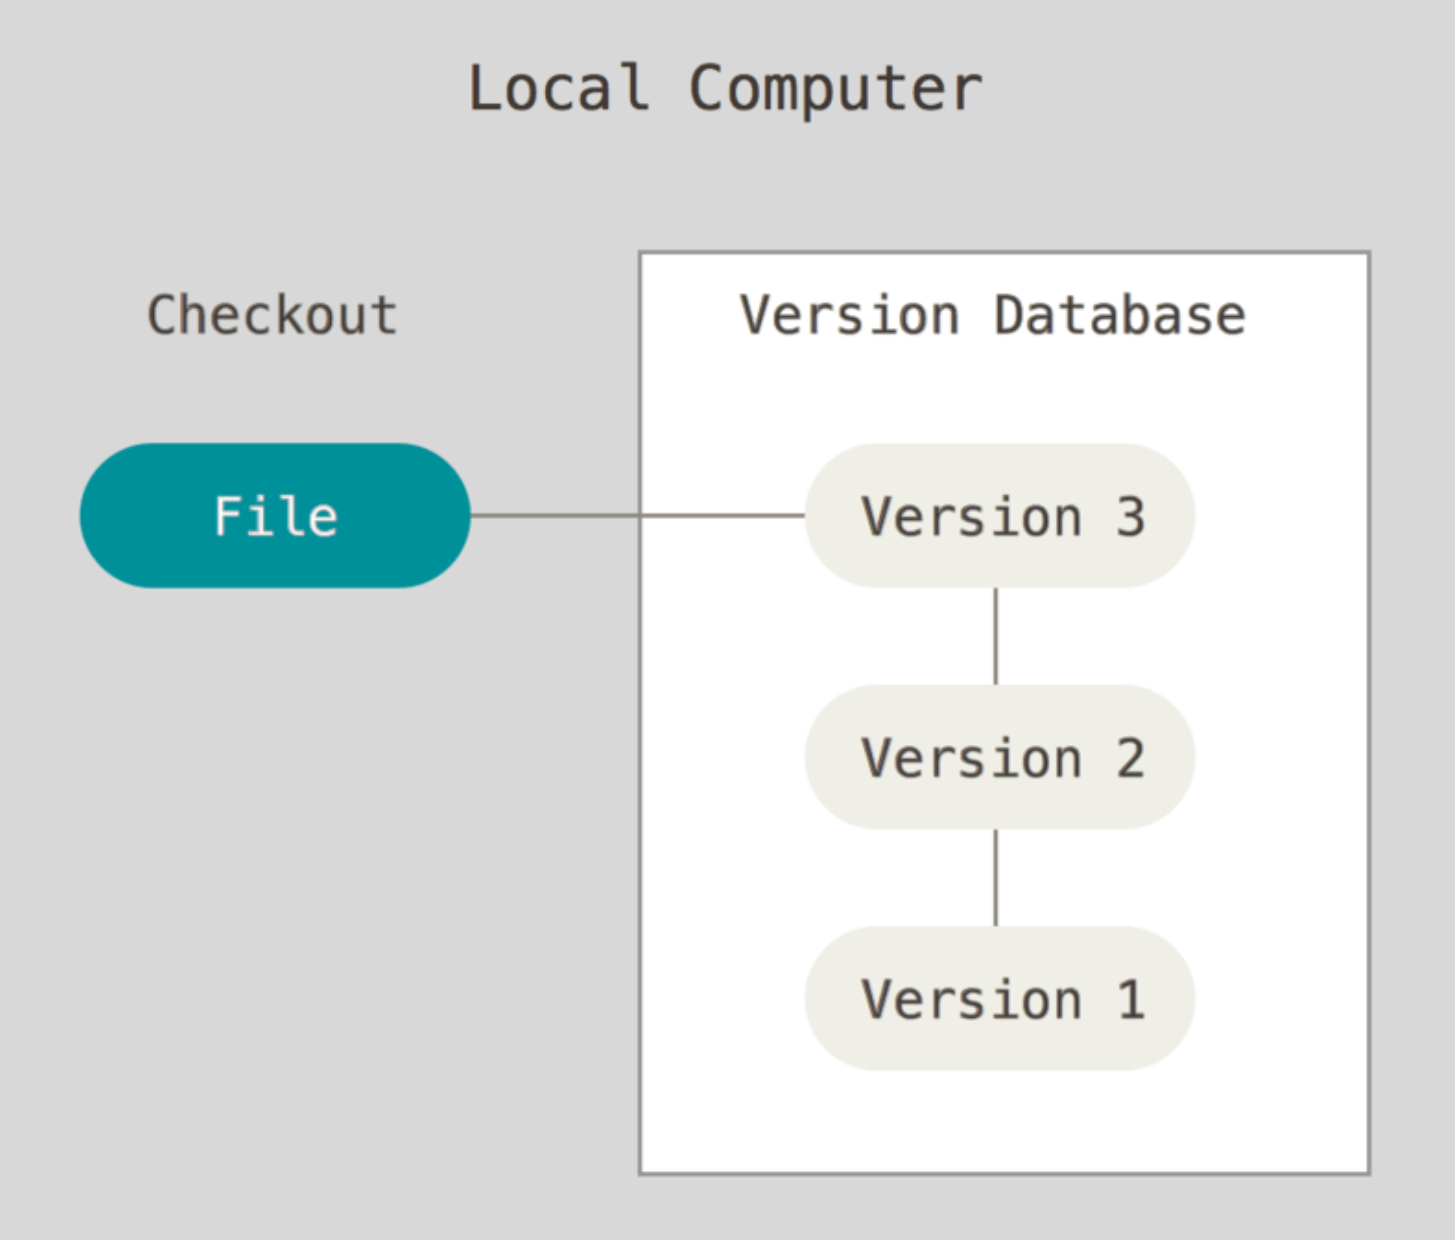
\includegraphics[width=0.6\textwidth]{localCopies.png}
			\attribution{https://git-scm.com/book/ru}
		\end{center}
	\end{frame}

	\begin{frame}
		\frametitle{Централизованные VCS}
		\begin{center}
			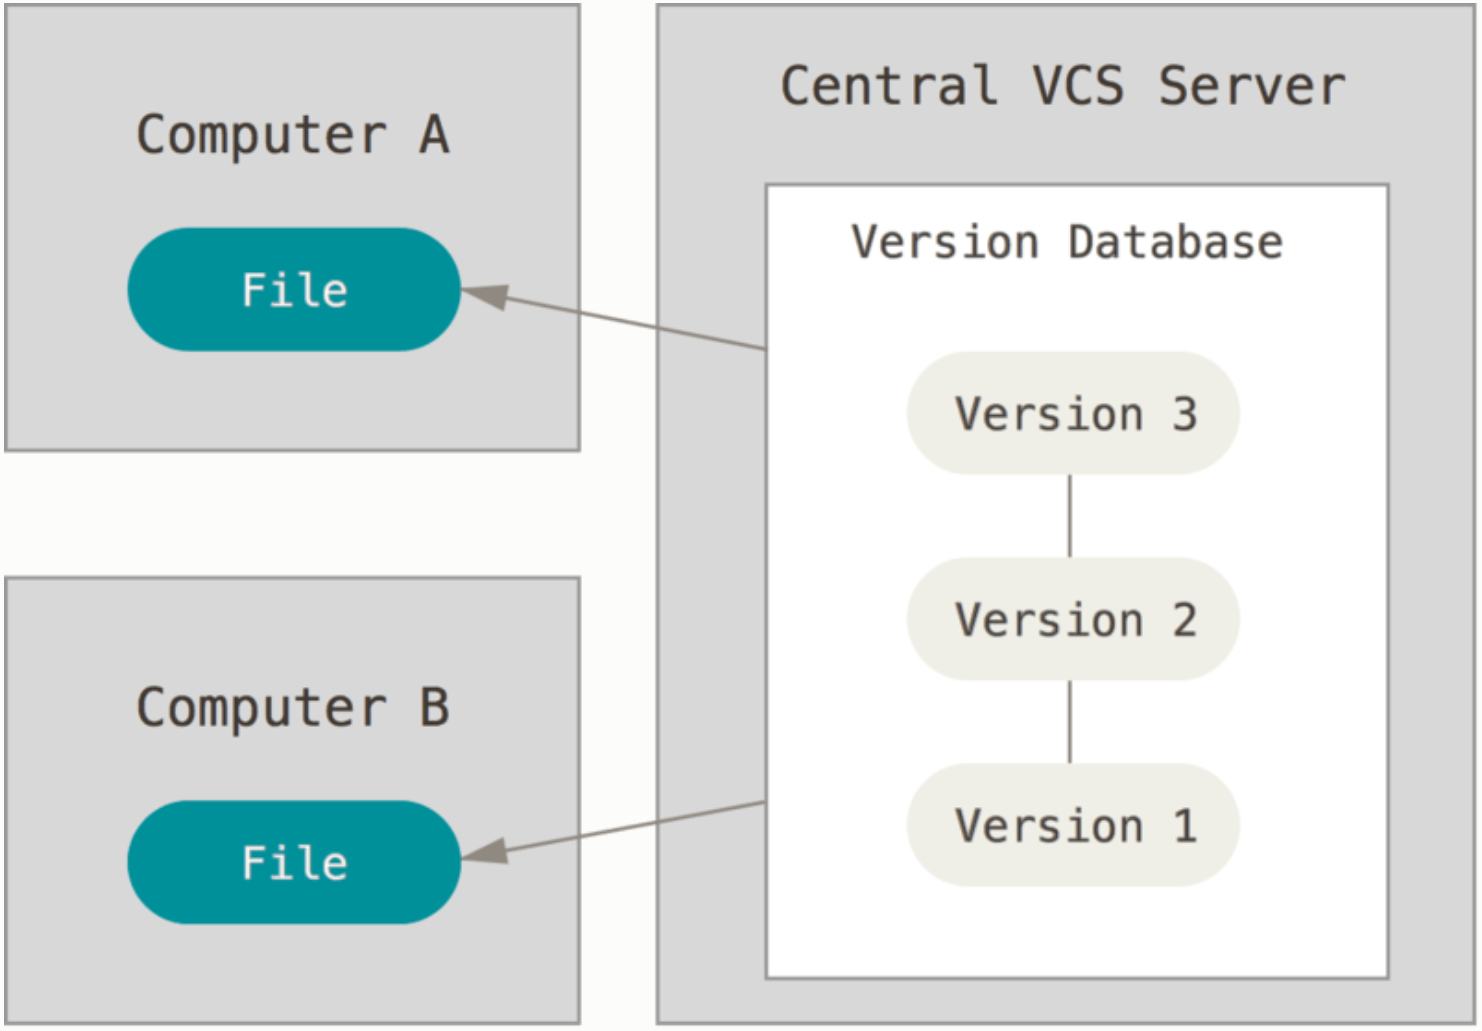
\includegraphics[width=0.6\textwidth]{centralizedVcs.png}
			\attribution{https://git-scm.com/book/ru}
		\end{center}
	\end{frame}

	\begin{frame}
		\frametitle{Распределенные VCS}
		\begin{center}
			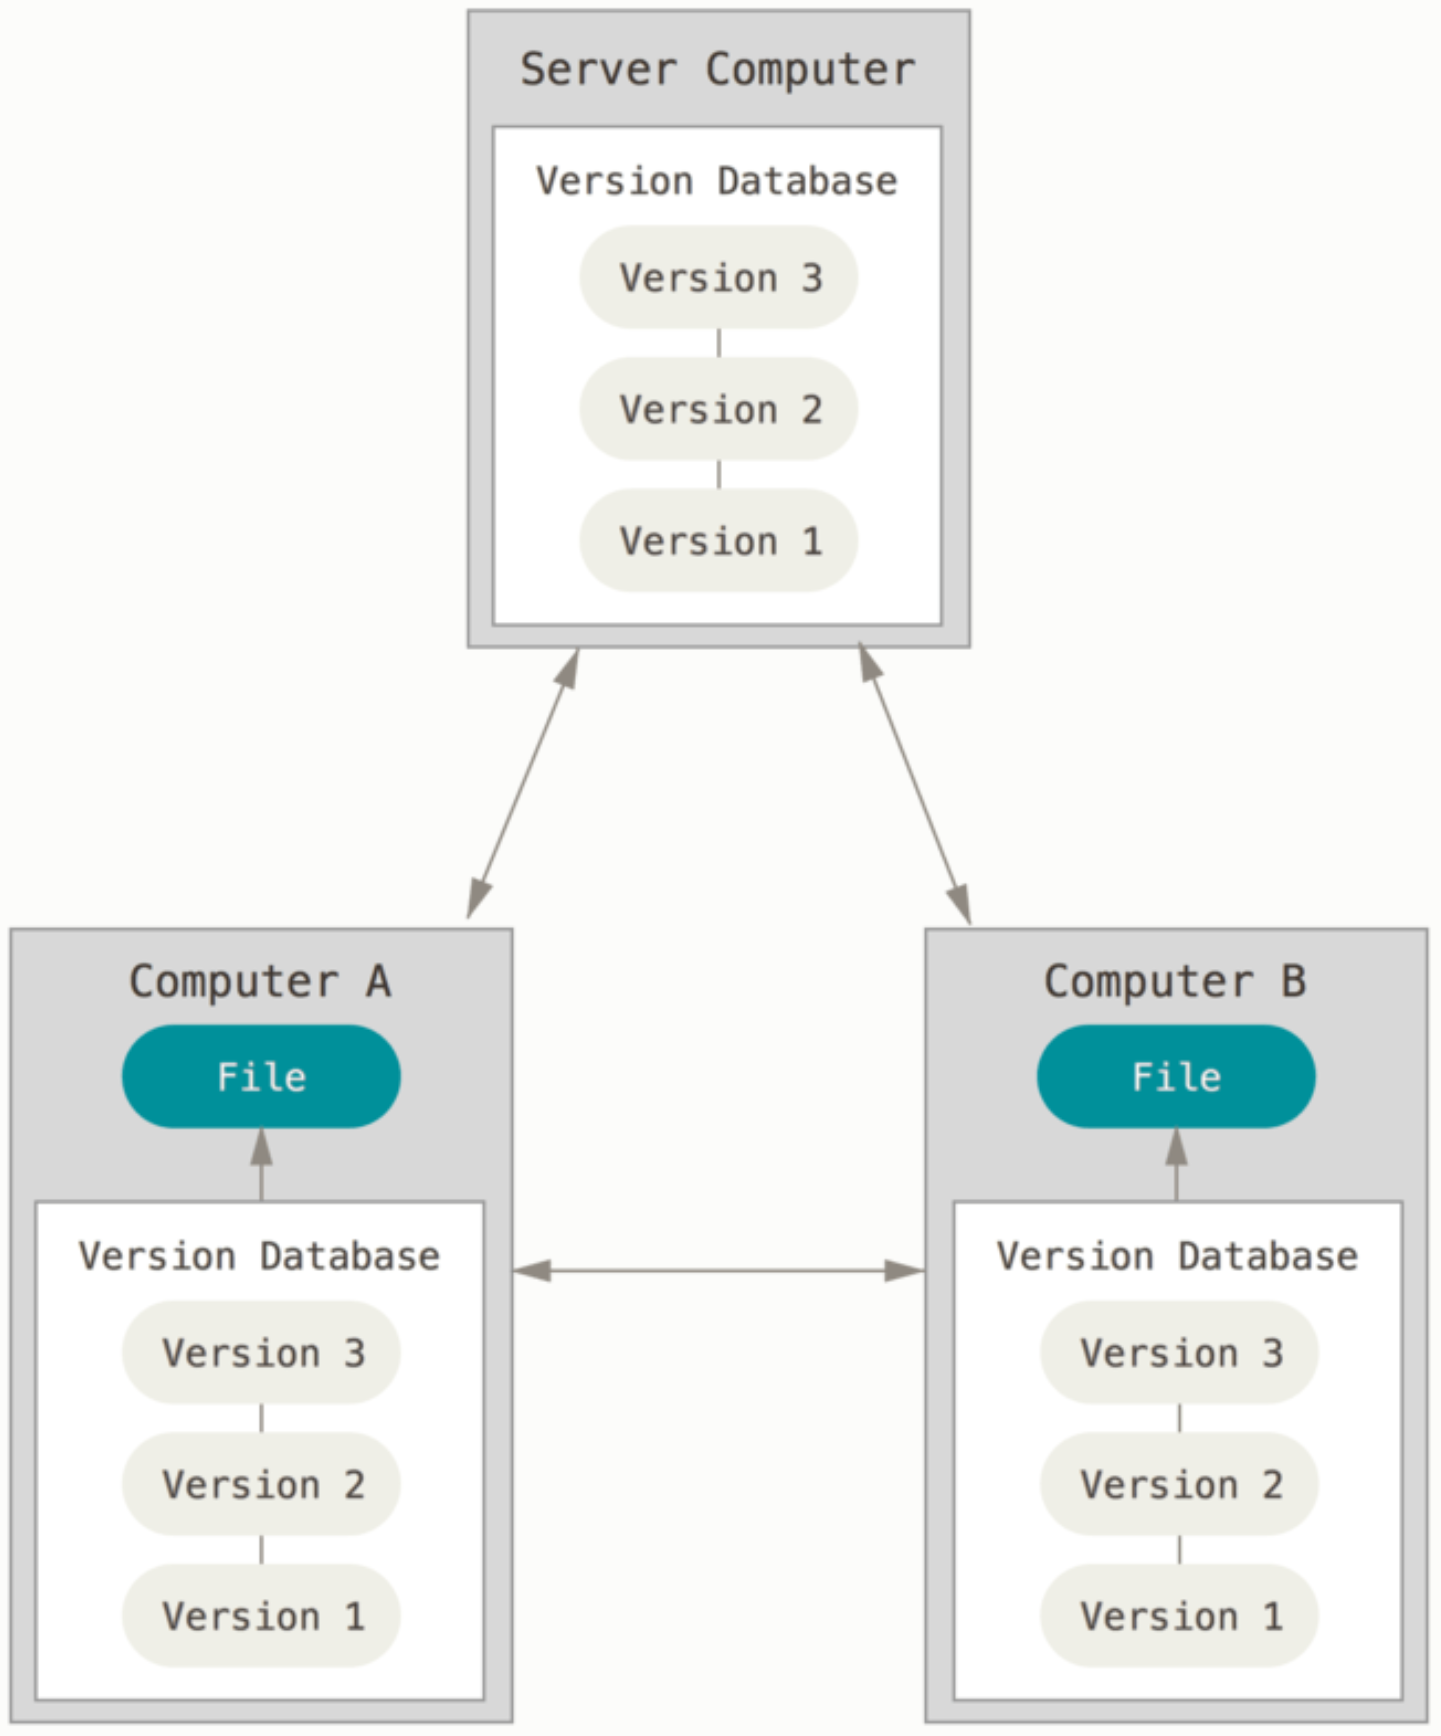
\includegraphics[width=0.4\textwidth]{distributedVcs.png}
			\attribution{https://git-scm.com/book/ru}
		\end{center}
	\end{frame}

	\begin{frame}
		\frametitle{Управление версиями}
		\begin{center}
			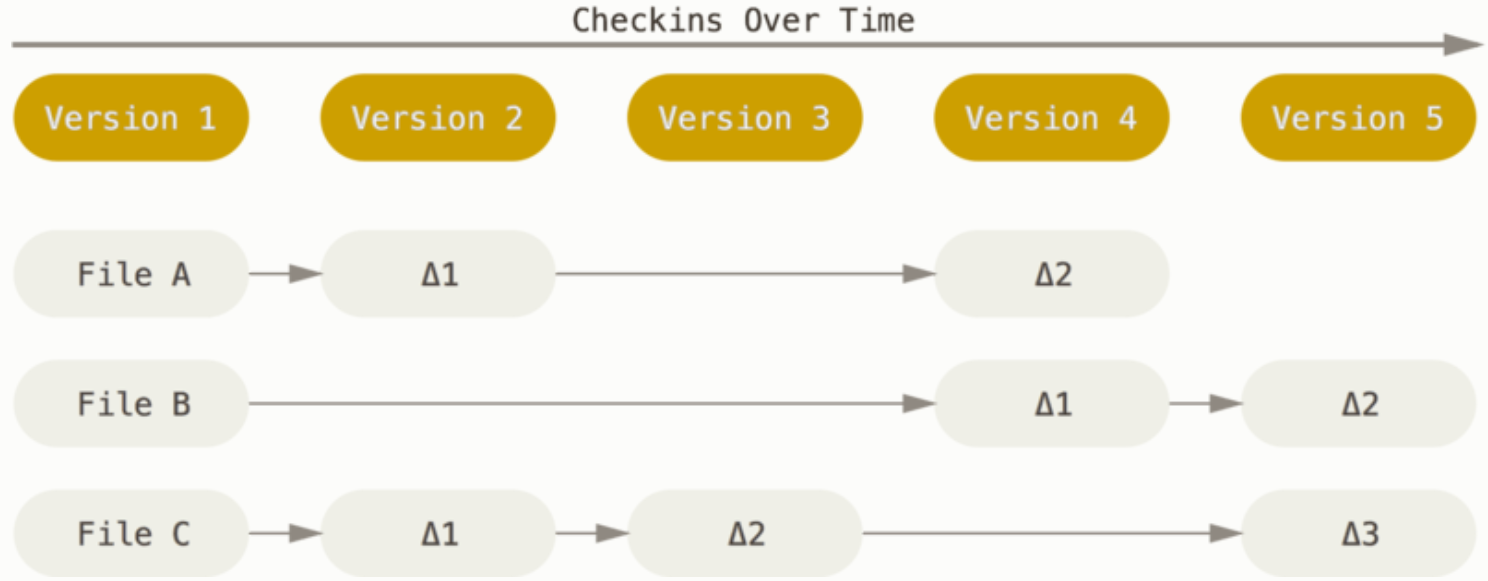
\includegraphics[width=0.6\textwidth]{deltaVersioning.png}

			\vspace{5mm}
			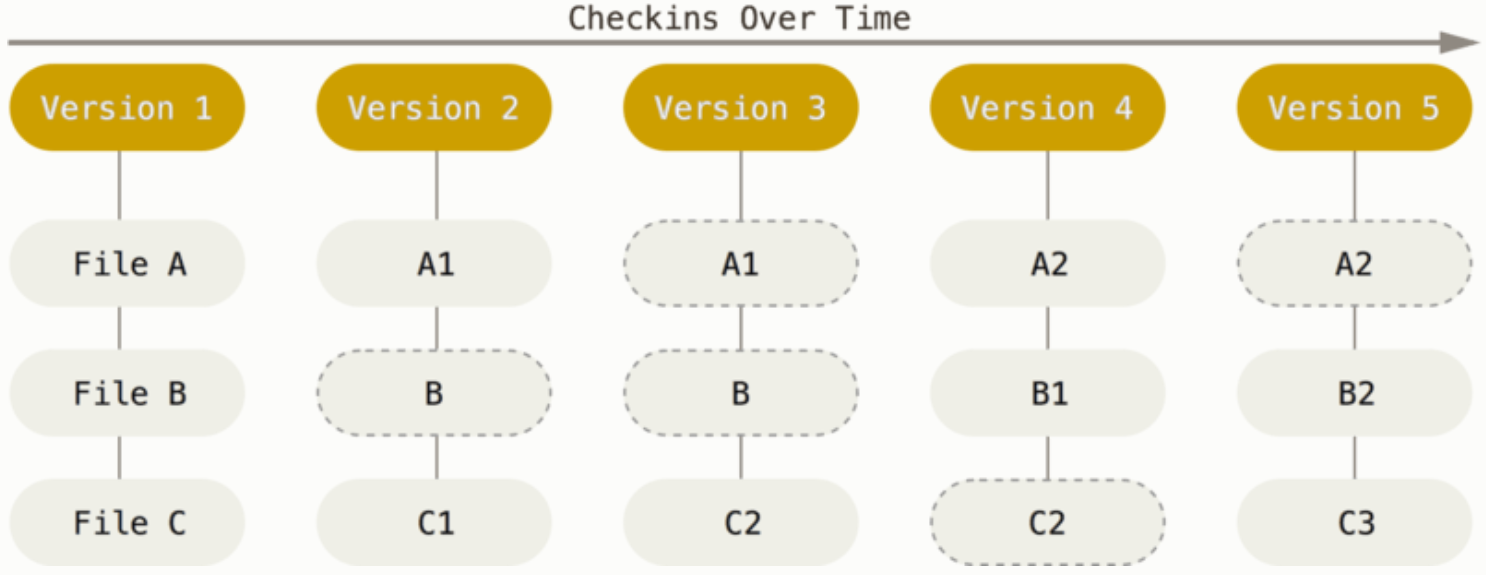
\includegraphics[width=0.6\textwidth]{snapshotVersioning.png}
			\attribution{https://git-scm.com/book/ru}
		\end{center}
	\end{frame}

	\begin{frame}
		\frametitle{Дельта}
		\begin{center}
			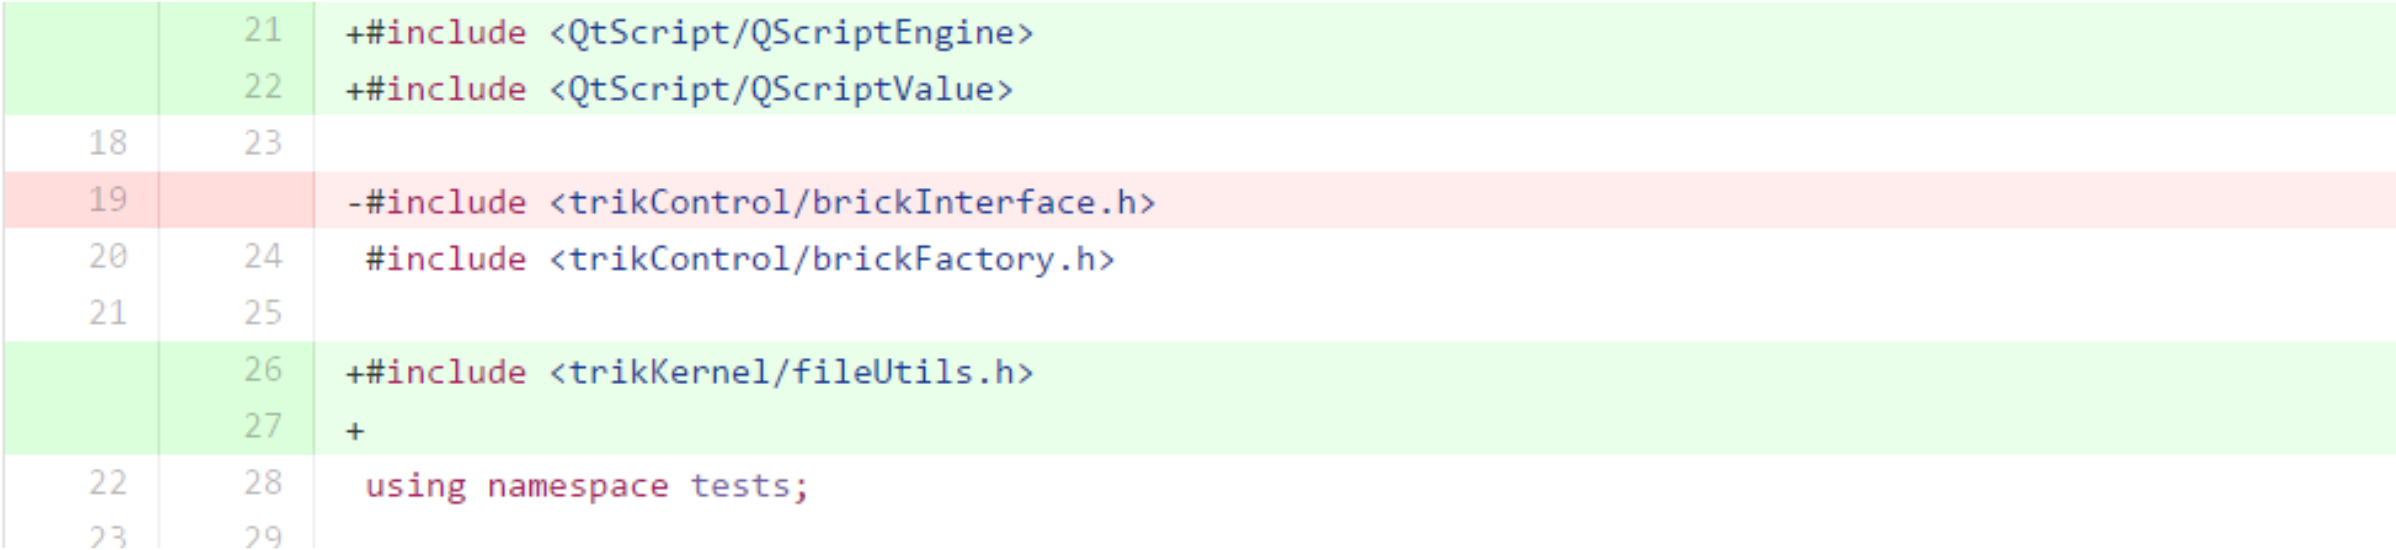
\includegraphics[width=0.8\textwidth]{delta.png}
		\end{center}
	\end{frame}

	\begin{frame}
		\frametitle{Жизненный цикл файла}
		\begin{center}
			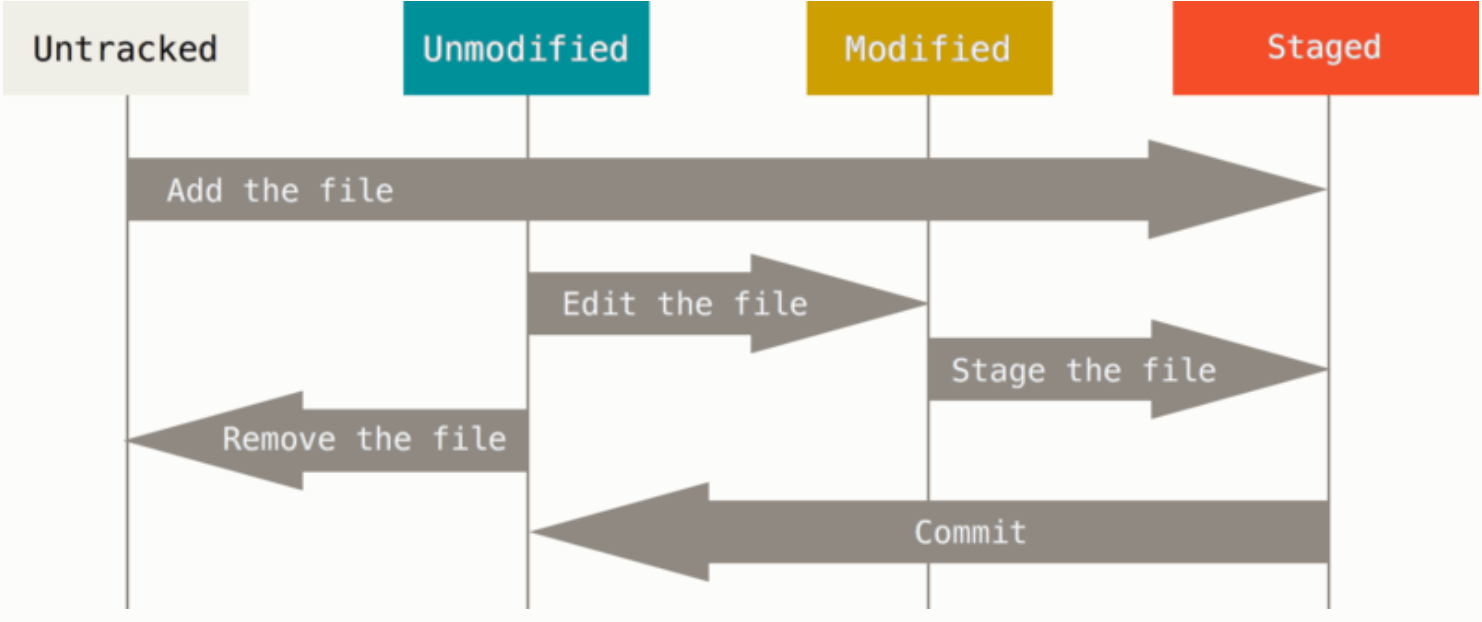
\includegraphics[width=0.8\textwidth]{fileLifeCycle.png}
			\attribution{https://git-scm.com/book/ru}
		\end{center}
	\end{frame}

	\begin{frame}
		\frametitle{Основные команды}
		\begin{itemize}
			\item git add --- добавить новый файл под управление git или добавить изменение к коммиту
			\item git status --- показать список изменённых/добавленных/удалённых файлов
			\item git diff --- показать изменения по каждому файлу
			\item git commit --- зафиксировать изменения, создав новый коммит
			\item git rm --- удалить файл и удалить его из репозиторий
			\item git log --- просмотреть список коммитов
			\item git checkout --- откатить изменения в файле или перейти на другую ветку
		\end{itemize}
	\end{frame}

	\begin{frame}[fragile]
		\frametitle{Как всё устроено}
		\begin{minted}{text}
$ git add README test.rb LICENSE
$ git commit -m 'initial commit of my project'
		\end{minted}
		\begin{center}
			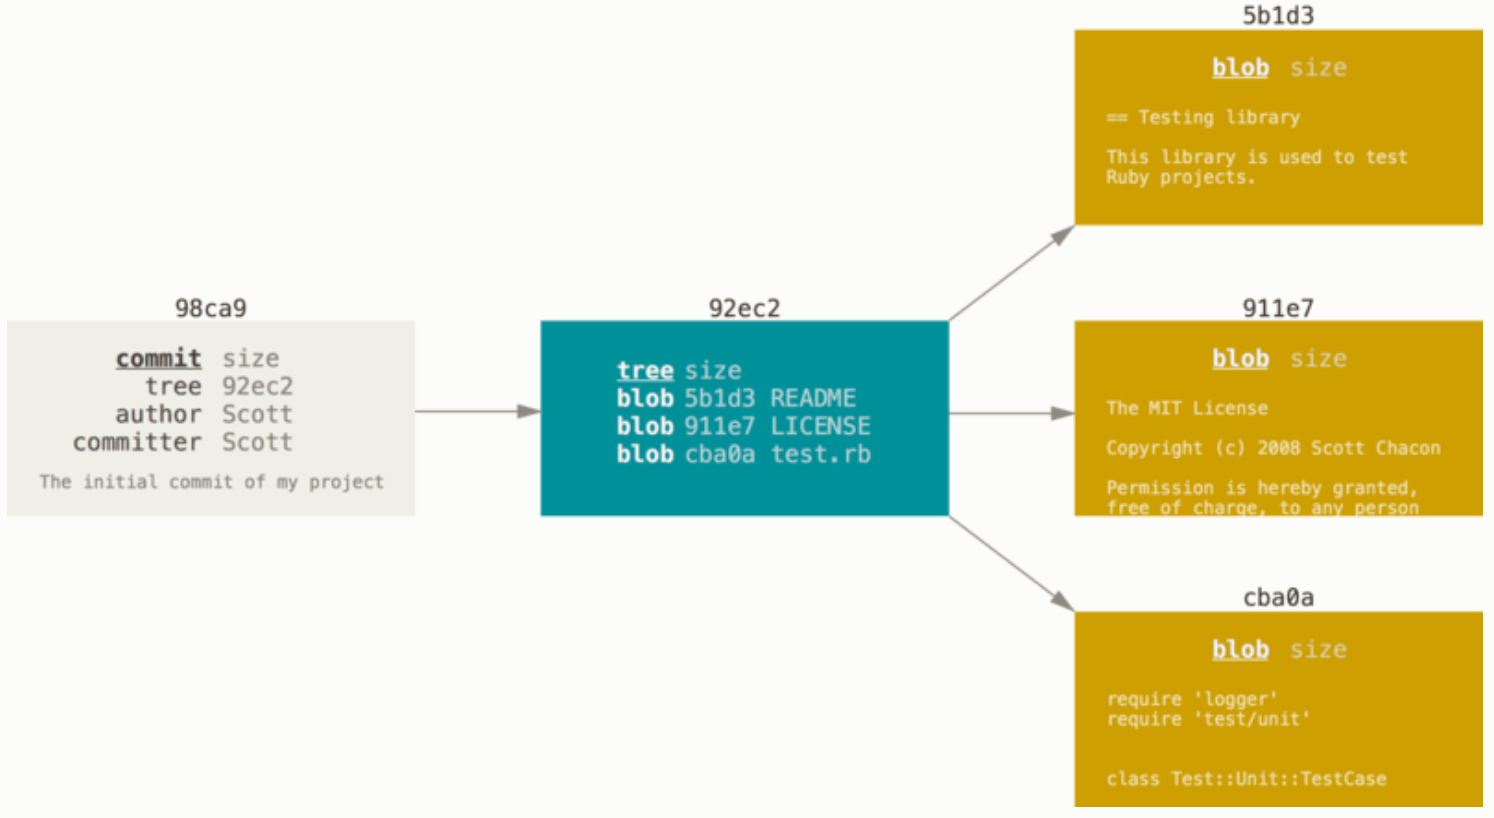
\includegraphics[width=0.8\textwidth]{blobs.png}
			\attribution{https://git-scm.com/book/ru}
		\end{center}
	\end{frame}

	\begin{frame}
		\frametitle{Коммит и его родители}
		\begin{center}
			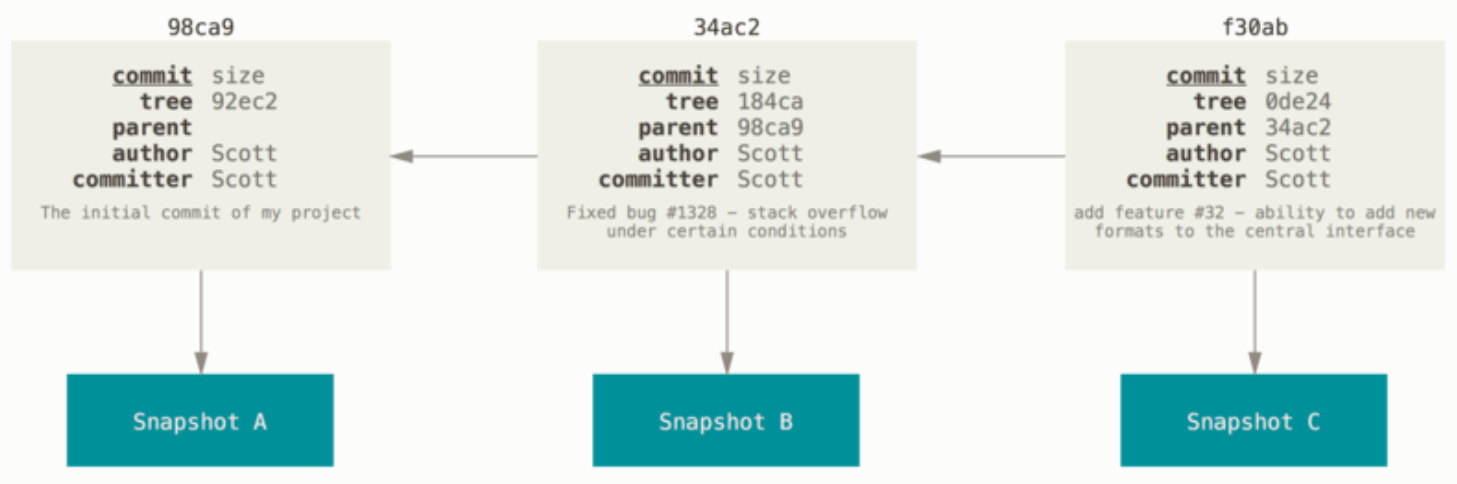
\includegraphics[width=0.8\textwidth]{commits.png}
			\attribution{https://git-scm.com/book/ru}
		\end{center}
	\end{frame}

	\begin{frame}
		\frametitle{Ветки}
		\begin{center}
			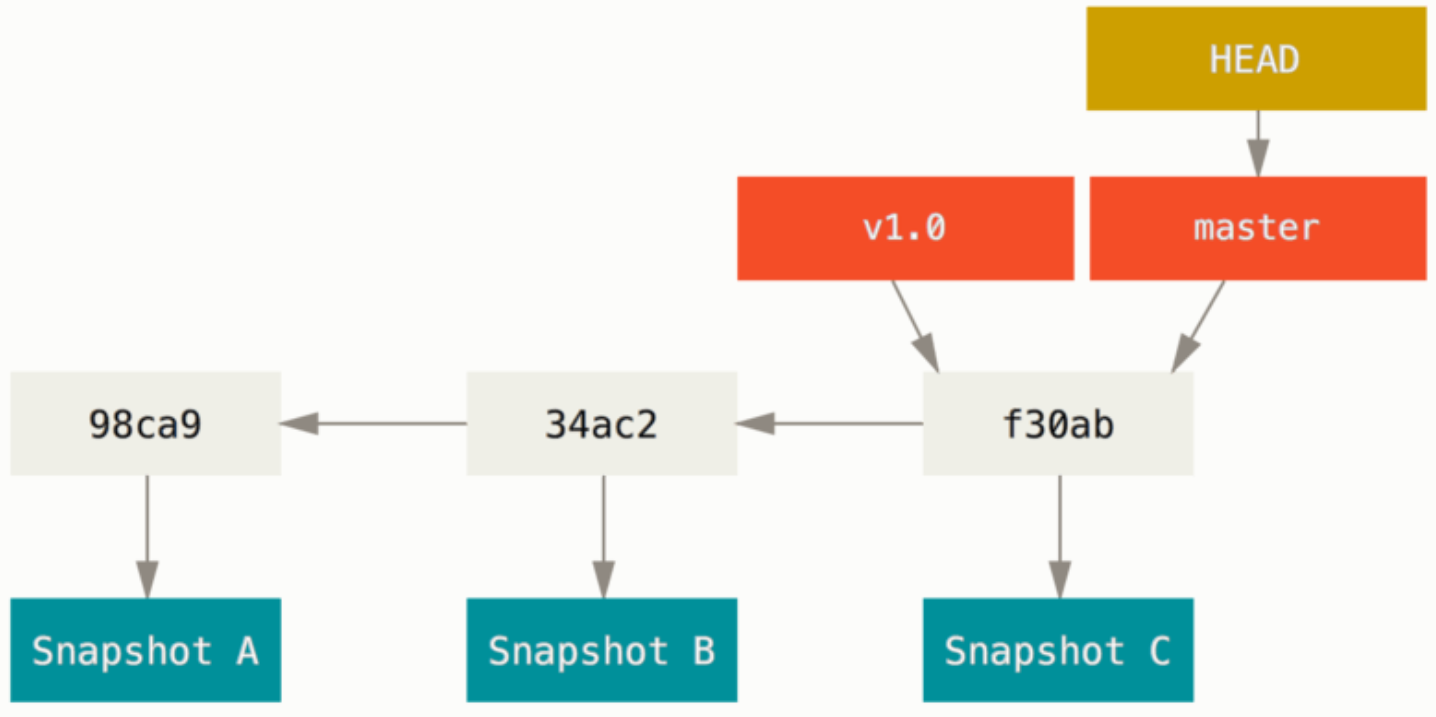
\includegraphics[width=0.8\textwidth]{branches.png}
			\attribution{https://git-scm.com/book/ru}
		\end{center}
	\end{frame}

	\begin{frame}[fragile]
		\frametitle{Создание ветки}
		\begin{minted}{text}
$ git branch testing
		\end{minted}
		\begin{center}
			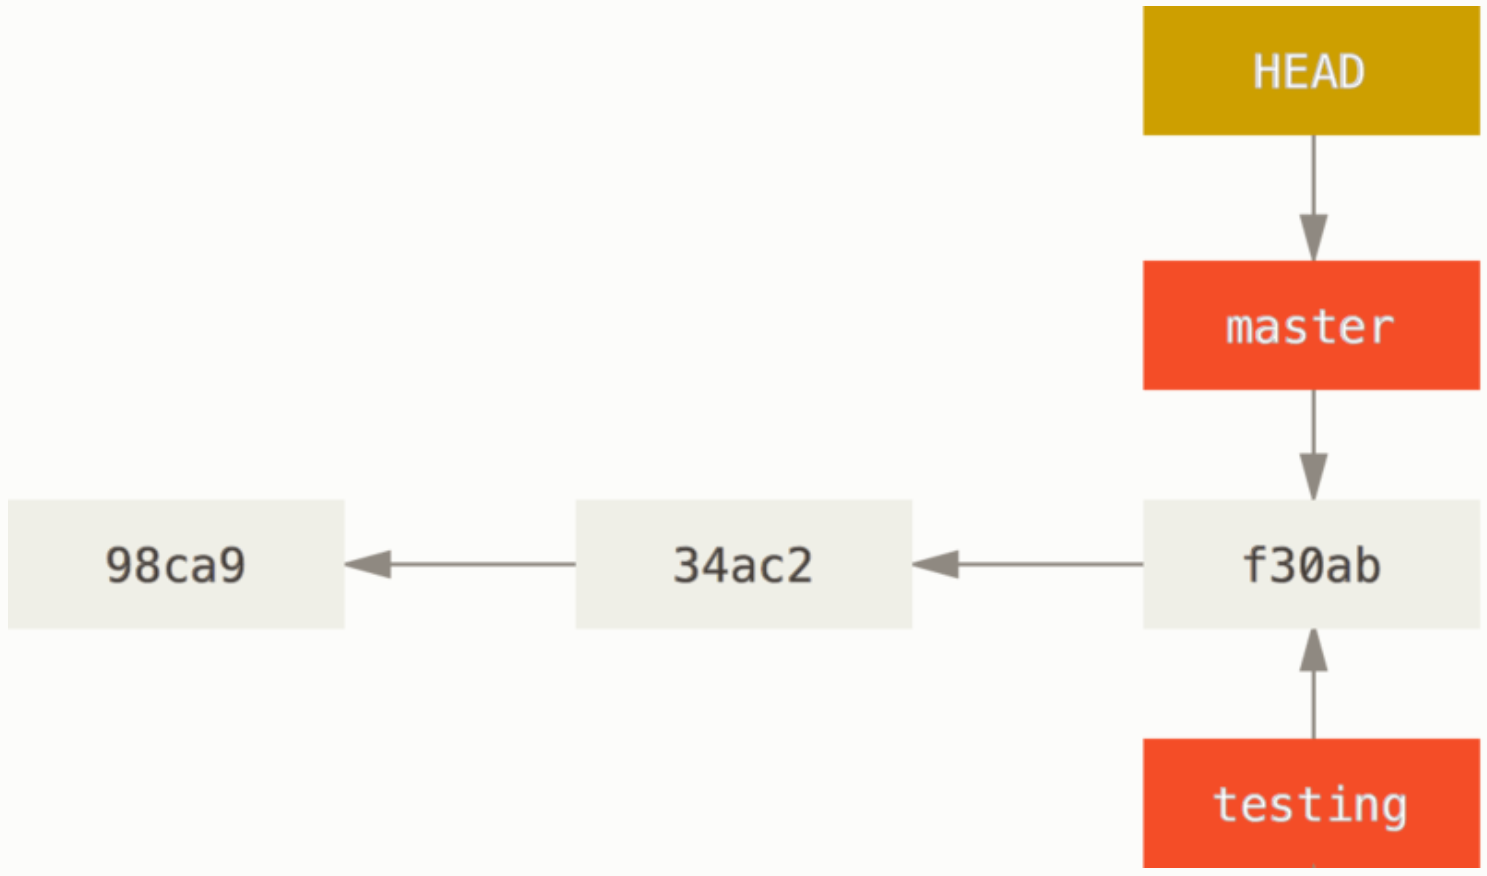
\includegraphics[width=0.8\textwidth]{creatingBranch.png}
			\attribution{https://git-scm.com/book/ru}
		\end{center}
	\end{frame}

	\begin{frame}[fragile]
		\frametitle{Переключение ветки}
		\begin{minted}{text}
$ git checkout testing
		\end{minted}
		\begin{center}
			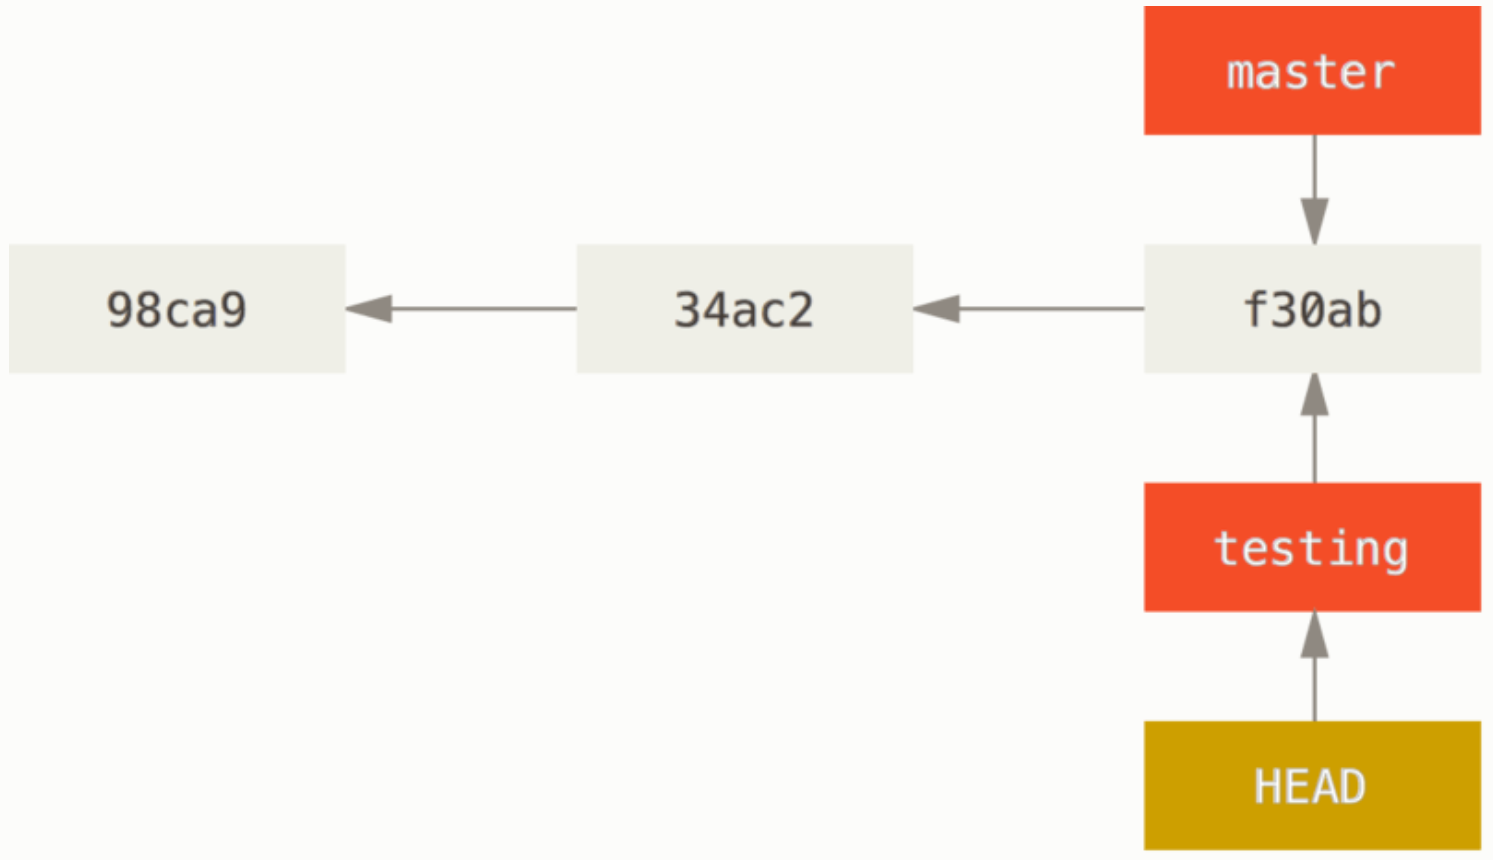
\includegraphics[width=0.8\textwidth]{checkout.png}
			\attribution{https://git-scm.com/book/ru}
		\end{center}
	\end{frame}

	\begin{frame}[fragile]
		\frametitle{Новый коммит}
		\begin{minted}{text}
<Что-то поделали с файлами в рабочей копии>
$ git add <изменения, которые хотим коммитить>
$ git commit -m 'made a change'
		\end{minted}
		\begin{center}
			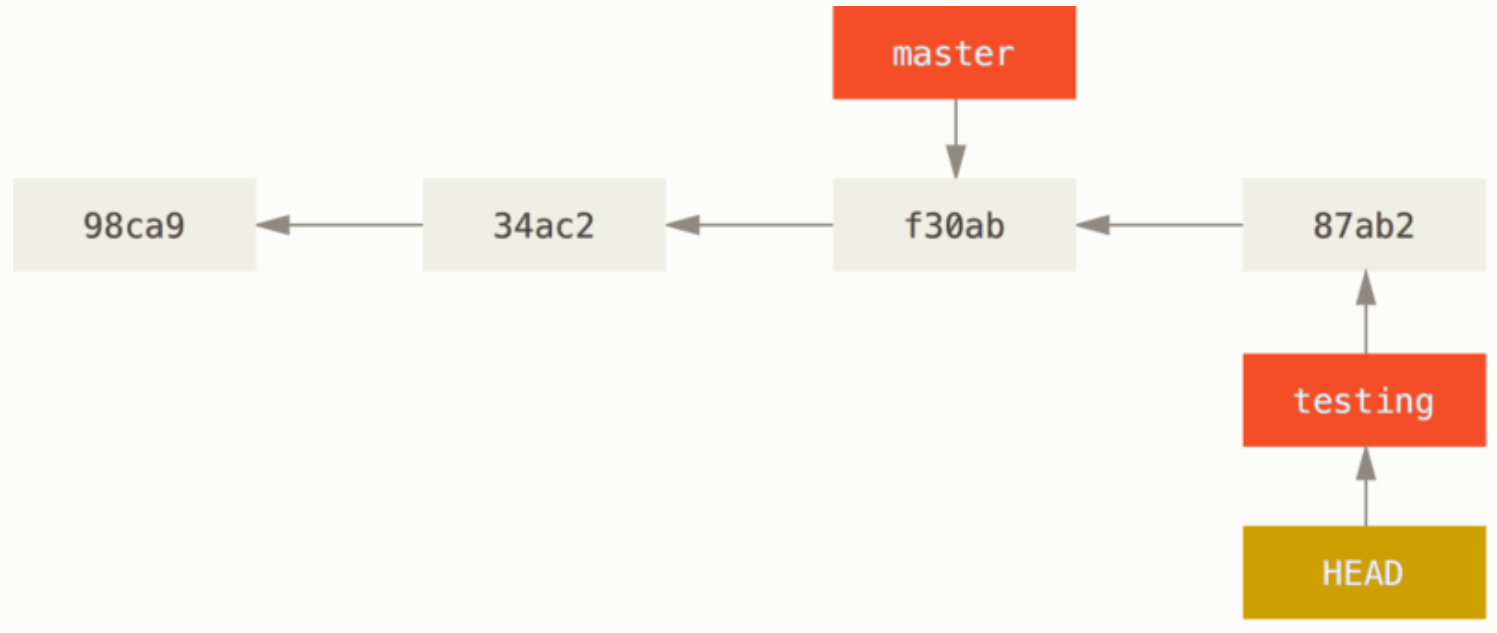
\includegraphics[width=0.8\textwidth]{newCommit.png}
			\attribution{https://git-scm.com/book/ru}
		\end{center}
	\end{frame}

	\begin{frame}[fragile]
		\frametitle{Переключимся на master}
		\begin{minted}{text}
$ git checkout master
		\end{minted}
		\begin{center}
			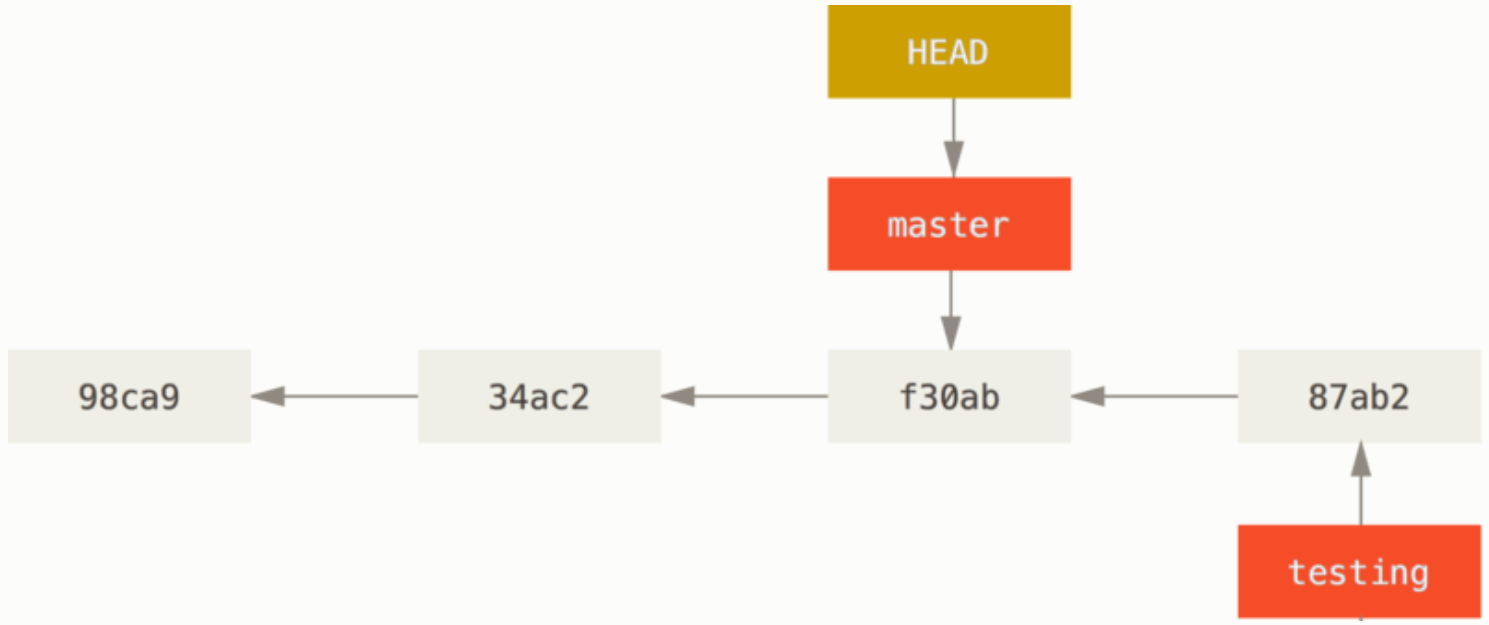
\includegraphics[width=0.8\textwidth]{checkoutToMaster.png}
			\attribution{https://git-scm.com/book/ru}
		\end{center}
	\end{frame}

	\begin{frame}[fragile]
		\frametitle{Сделаем новый коммит там}
		\begin{minted}{text}
<Что-то поделали с файлами в рабочей копии>
$ git add <изменения, которые хотим коммитить>
$ git commit -m 'made other changes'
		\end{minted}
		\begin{center}
			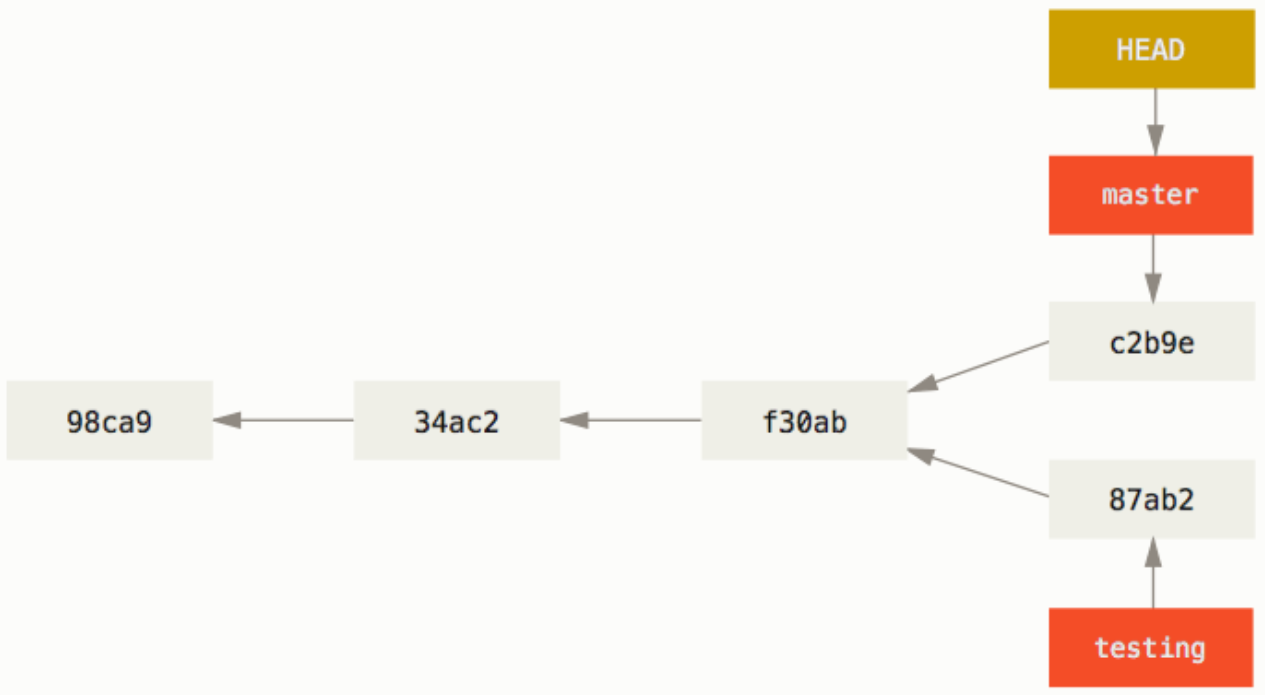
\includegraphics[width=0.8\textwidth]{newCommitToMaster.png}
			\attribution{https://git-scm.com/book/ru}
		\end{center}
	\end{frame}

	\begin{frame}[fragile]
		\frametitle{Слияние веток}
		\begin{minted}{text}
$ git checkout master
Switched to branch 'master'
$ git merge testing
Merge made by the 'recursive' strategy.
index.html |    1 +
1 file changed, 1 insertion(+)
		\end{minted}
		\begin{center}
			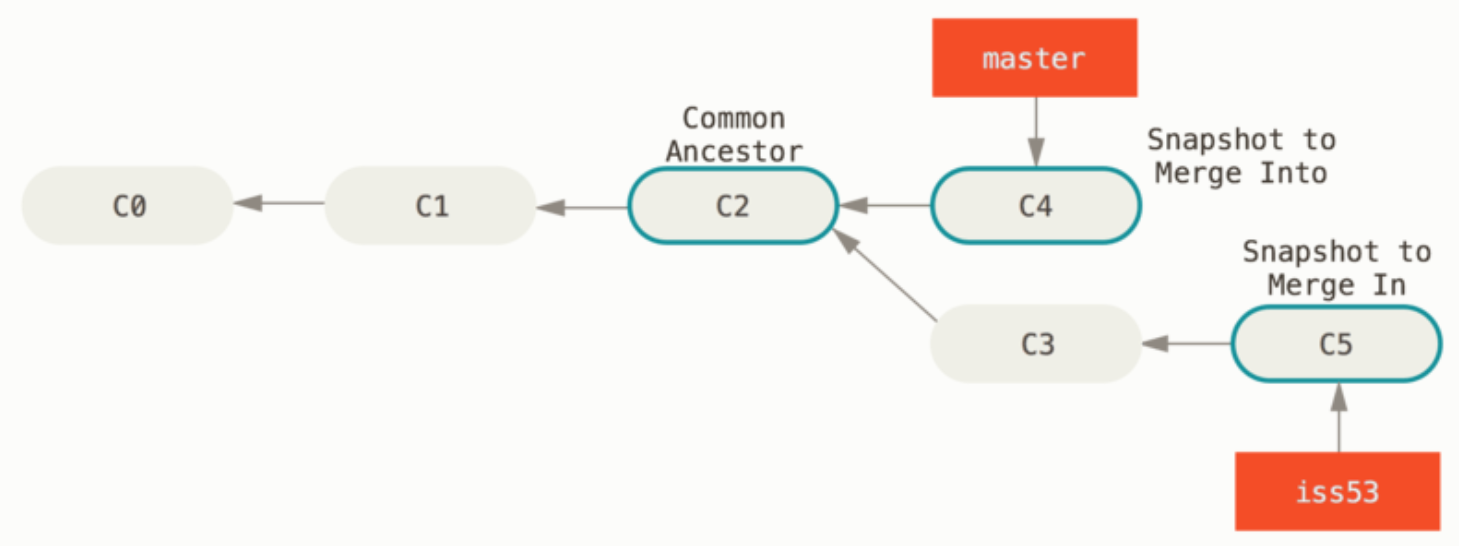
\includegraphics[width=0.8\textwidth]{merge.png}
			\attribution{https://git-scm.com/book/ru}
		\end{center}
	\end{frame}

	\begin{frame}
		\frametitle{Результат}
		\begin{center}
			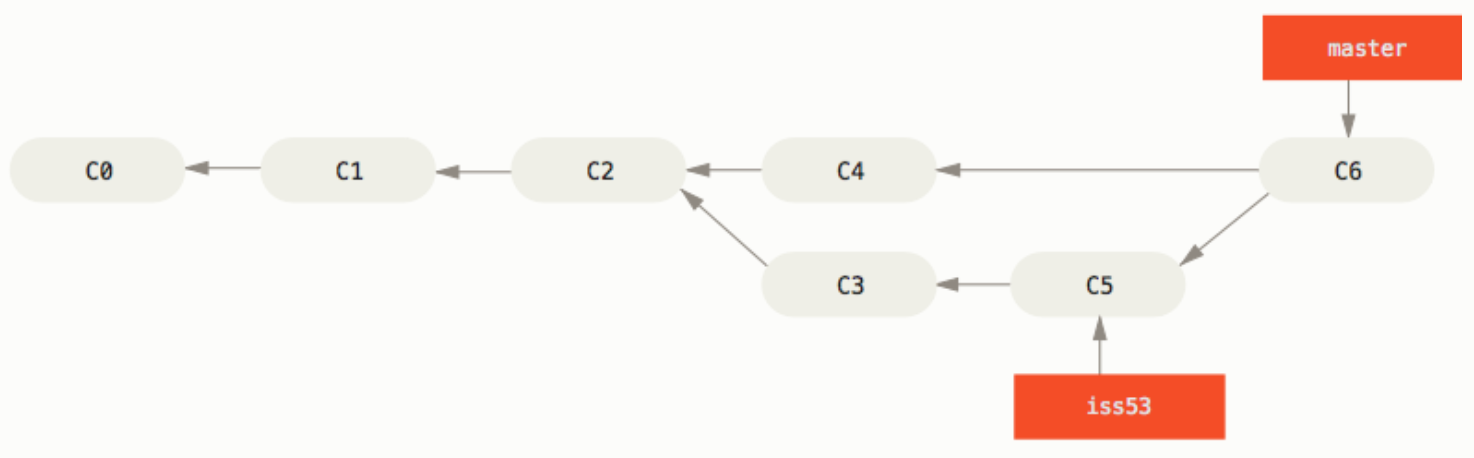
\includegraphics[width=0.8\textwidth]{mergeResult.png}
			\attribution{https://git-scm.com/book/ru}
		\end{center}
	\end{frame}

	\begin{frame}
		\frametitle{Конфликты}
		\begin{center}
			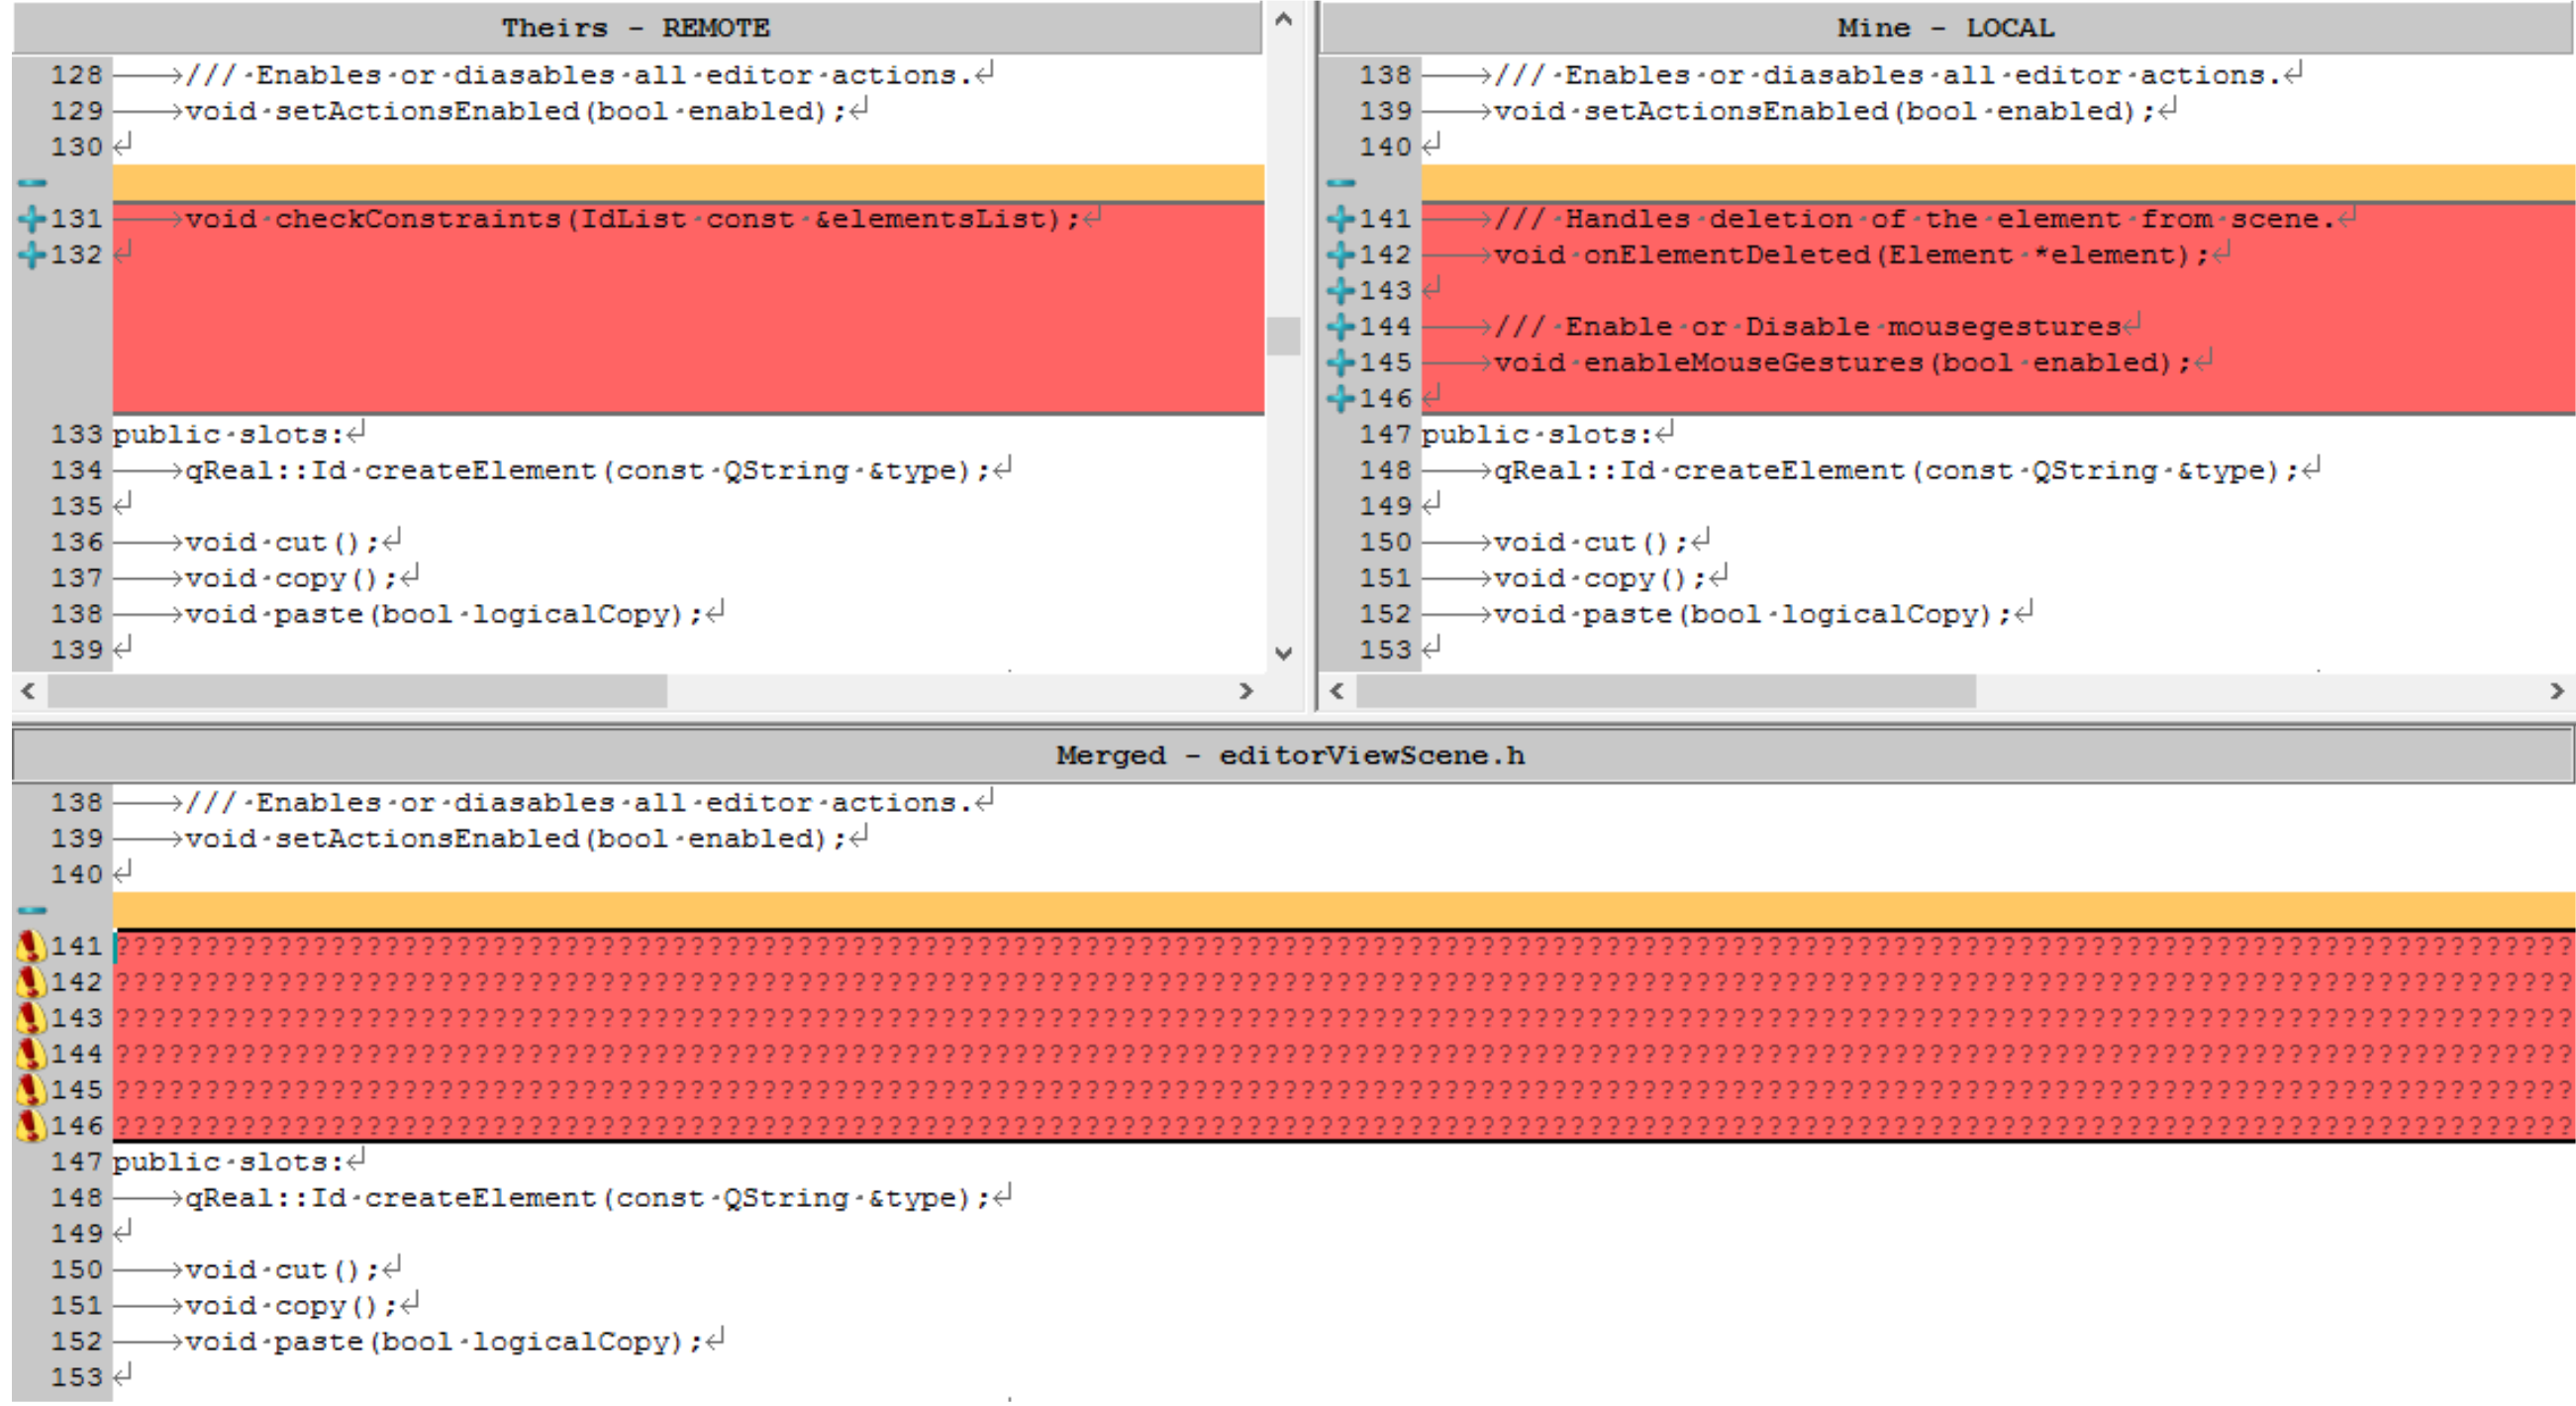
\includegraphics[width=0.95\textwidth]{conflicts.png}
		\end{center}
	\end{frame}

	\begin{frame}
		\frametitle{Конфликты в коде}
		\begin{center}
			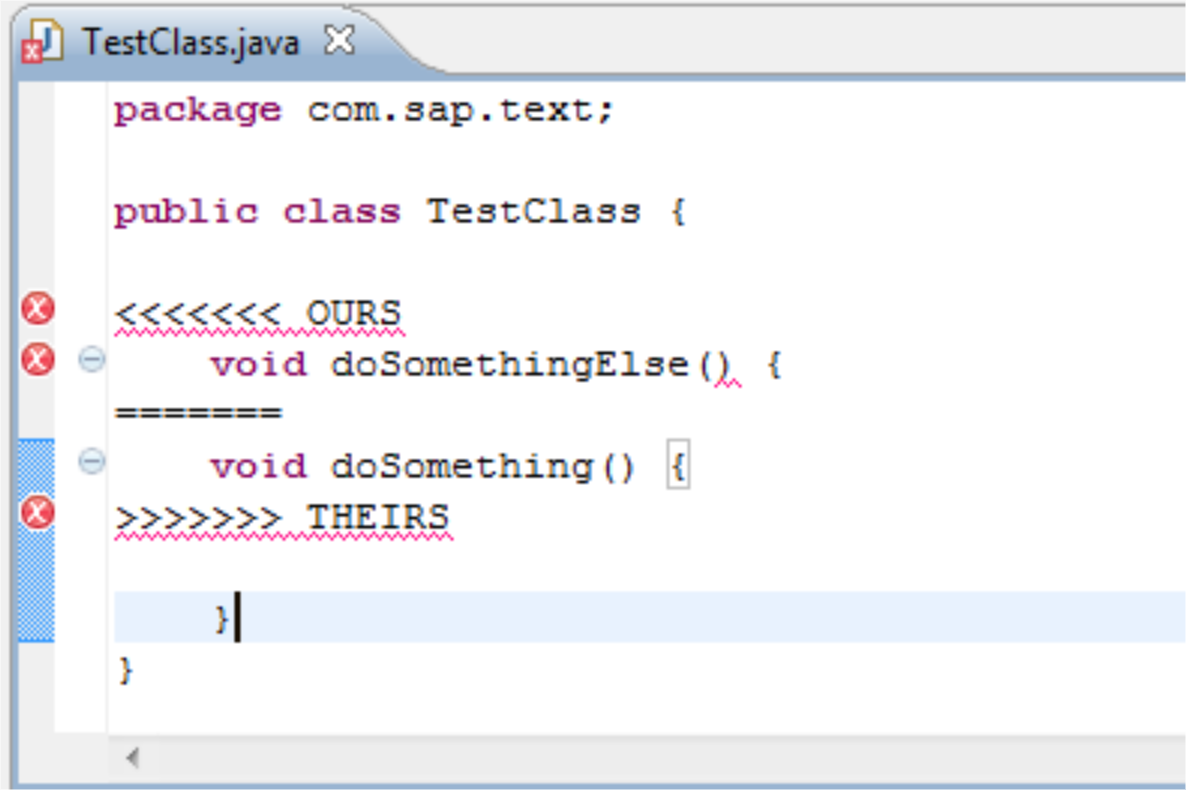
\includegraphics[width=0.5\textwidth]{conflictsInCode.png}
		\end{center}
	\end{frame}

	\begin{frame}
		\frametitle{Удалённые репозитории}
		\begin{columns}
			\begin{column}{0.4\textwidth}
				\begin{itemize}
					\item git clone
					\item git remote
					\item git push
					\item git fetch
					\item git pull
				\end{itemize}
			\end{column}
			\begin{column}{0.6\textwidth}
				\begin{center}
					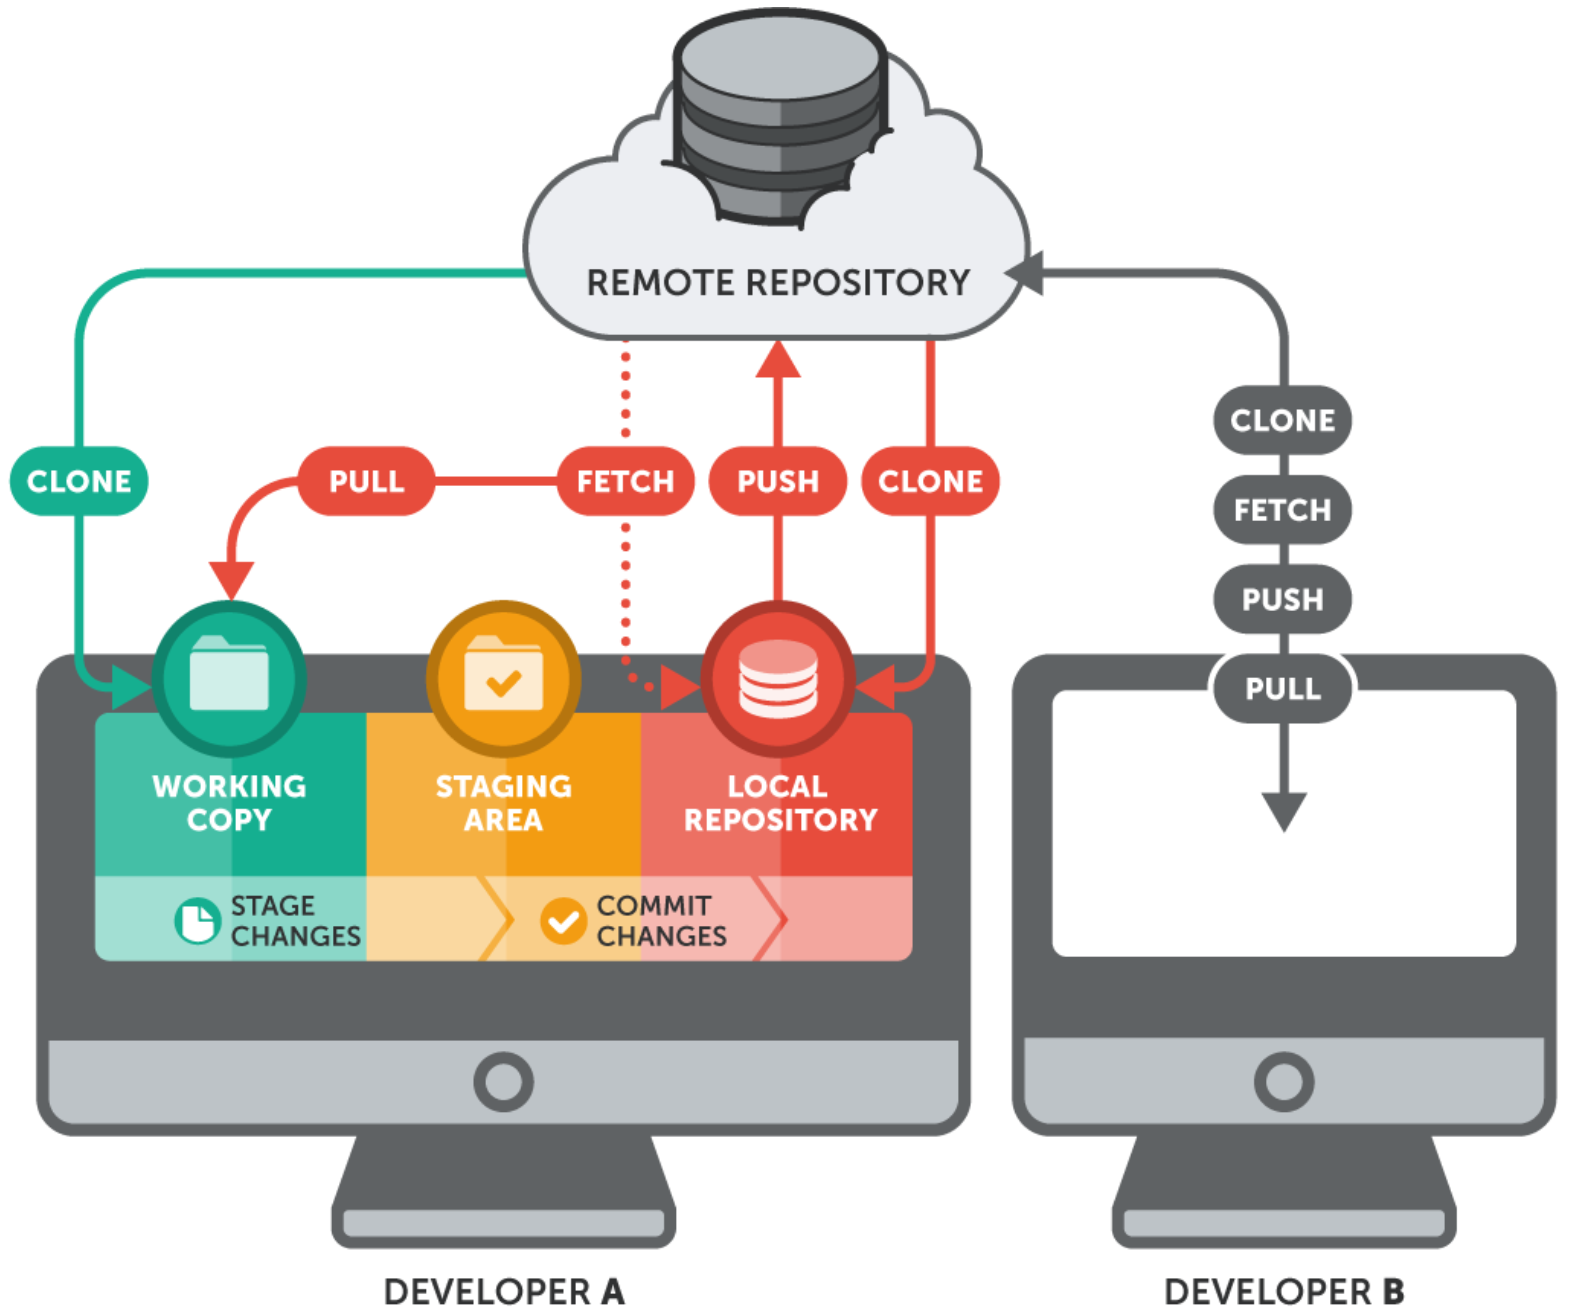
\includegraphics[width=0.95\textwidth]{remoteRepos.png}
					\attribution{https://www.git-tower.com/learn/git/ebook/en}
				\end{center}
			\end{column}
		\end{columns}
	\end{frame}

	\begin{frame}
		\frametitle{Процесс работы}
		\begin{footnotesize}
			\begin{itemize}
				\item Программист хочет сделать новую фичу
				\item Отводит себе ветку от мастера
				\item Реализует там фичу
				\item Тестит и рефакторит её, когда считает, что она готова, делает пуллреквест
				\item Пока пуллреквест ревьюят, программист делает новую фичу (опять-таки, отведя новую ветку от мастера)
				\item По пуллреквесту появляются замечания, программист переключается на ветку пуллреквеста и правит там замечания
				\item Когда поправил, коммитит и пушит исправления, они автоматом добавляются в пуллреквест
				\item Просит ревьюеров, чтобы они посмотрели фиксы
				\item Переключается обратно на свою рабочую ветку и продолжает писать код, возможно, делая ещё пуллреквесты 
				\item Цикл повторяется до тех пор, пока пуллреквест не принимают
				\item Программист удаляет ветку с фичей, когда она замерджена
			\end{itemize}
		\end{footnotesize}
	\end{frame}

	\begin{frame}
		\frametitle{То же, но с домашкой}
		\begin{itemize}
			\item Хотите сделать новую задачу
			\item Отводите себе ветку от мастера
			\begin{itemize}
				\item git checkout master
				\item git branch my-cool-hometask-3.1
			\end{itemize}
			\item Создаёте \textbf{прямо там} проект, делаете задачу
			\item Коммитите, сколько хотите
			\begin{itemize}
				\item После каждого значимого продвижения
				\item git add на каждый новый файл, который надо коммитить
				\item git commit -a -m"Внятное описание изменений"
			\end{itemize}
		\end{itemize}
	\end{frame}

	\begin{frame}
		\frametitle{То же, но с домашкой (2)}
		\begin{itemize}
			\item Когда считаете, что задача готова, пушите её на гитхаб
			\begin{itemize}
				\item git push -u origin my-cool-hometask-3.1
			\end{itemize}
			\item Идёте на гитхаб, делаете пуллреквест
			\begin{itemize}
				\item Выбираете ветку в ``Branch:''
				\item Жмёте на Pull request
				\item Вводите внятное описание пуллреквеста
				\item Жмёте на Create pull request
			\end{itemize}
			\item Ссылку на то, что получилось, выкладываете на HwProj
			\begin{itemize}
				\item Список всех пуллреквестов можно посмотреть во вкладке Pull requests на гитхабе
			\end{itemize}
			\item Ждёте, пока я прокомментирую решение
		\end{itemize}
	\end{frame}

	\begin{frame}
		\frametitle{То же, но с домашкой (3)}
		\begin{itemize}
			\item В это время можно заняться следующей задачей
			\begin{itemize}
				\item Не забыть git checkout master
				\item git branch my-cool-hometask-3.2
			\end{itemize}
			\item Получаете ревью на гитхабе, исправляете замечания
			\begin{itemize}
				\item Переключаетесь на исходную ветку
				\begin{itemize}
					\item Коммитите текущие изменения в рабочей копии
					\item git checkout my-cool-hometask-3.1
				\end{itemize}
				\item Исправляете, коммитя сколько хотите
				\item Коммитите исправления
				\item Пушите на гитхаб
				\begin{itemize}
					\item git push, без всяких -u
				\end{itemize}
			\end{itemize}
			\item Проверяете, что всё ок, в пуллреквестах на гитхабе
			\item Когда задача принята, мерджите пуллреквест на гитхабе и удаляете ветку
		\end{itemize}
	\end{frame}

	\begin{frame}
		\frametitle{Что надо выкладывать}
		\begin{itemize}
			\item .cpp, .h-файлы
			\item Проектные файлы:
			\begin{itemize}
				\item Visual Studio: .vcxproj, .sln
				\item Qt Creator: .pro
				\item CLion: всё содержимое папки .idea, кроме workspace.xml и tasks.xml
			\end{itemize}
			\item Текстовые файлы и прочие ресурсы, которые используются в тестах или во время работы программы
		\end{itemize}
	\end{frame}

	\begin{frame}
		\frametitle{Что не надо выкладывать}
		\begin{itemize}
			\item Бинарные файлы: .exe, .dll, бинарники под линуксом
			\begin{itemize}
				\item Включите себе отображение расширений файлов
			\end{itemize}
			\item Промежуточные результаты компиляции: .o, .obj, ...
			\item Скрытую папку .vs в Visual Studio
			\begin{itemize}
				\item Включите себе отображение скрытых файлов
			\end{itemize}
			\item Makefile-ы и подобные вещи в Qt Creator
		\end{itemize}
		.gitignore:
		\begin{itemize}
			\item \url{https://git-scm.com/docs/gitignore}
			\item \url{https://github.com/github/gitignore}
		\end{itemize}
	\end{frame}

	\begin{frame}
		\frametitle{Хорошие практики}
		\begin{itemize}
			\item Аккуратно заполняем Имя и Email
			\begin{itemize}
				\item Желательно, чтобы они совпадали с именем аккаунта и почтой, с которой регались на гитхабе
			\end{itemize}
			\item Коммитим только то, что нужно, чтобы получить в чистую папку и собрать проект
			\item Всегда пишем адекватные комментарии к коммитам
			\item Коммитим как можно чаще
			\item Один коммит --- одна функциональность
			\begin{itemize}
				\item Сделали что-то, хоть немного напоминающее осмысленное -> коммит
			\end{itemize}
		\end{itemize}
	\end{frame}

	\begin{frame}
		\frametitle{Хорошие практики (2)}
		\begin{itemize}
			\item Коммит не должен содержать в себе файлы, не относящиеся к изменениям
			\begin{itemize}
				\item .gitignore
			\end{itemize}
			\item Коммит не должен добавлять/убирать пустые строки, менять пробелы на табы и т.д., если это не суть коммита
			\item Стиль исходного кода и отступов должен совпадать с текстом вокруг
		\end{itemize}
		\begin{center}
			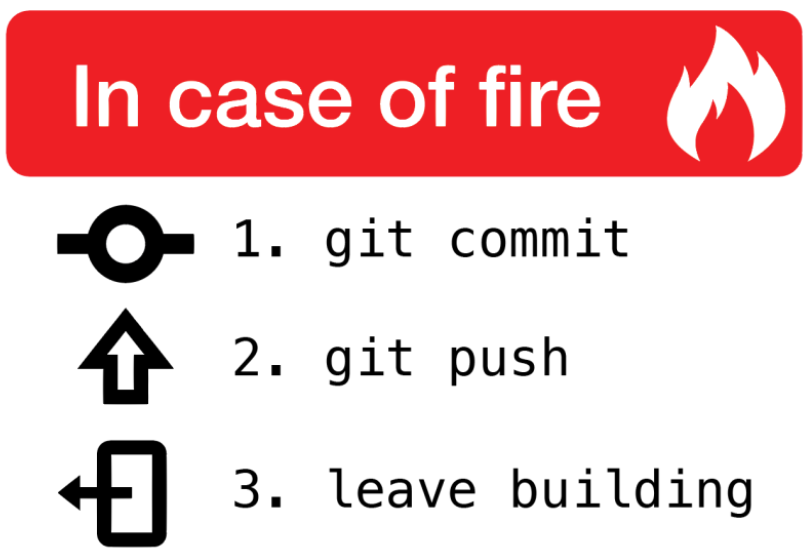
\includegraphics[width=0.4\textwidth]{inCaseOfFire.png}
		\end{center}
	\end{frame}

	\begin{frame}[fragile]
		\frametitle{Ещё полезные команды}
		\begin{itemize}
			\item \verb|git add -p| --- интерактивное добавление изменений к коммиту, позволяет коммитить только часть файла
			\item \verb|git commit --amend| --- исправить последний коммит
			\begin{itemize}
				\item \verb|git commit --amend -m "an updated commit message"|
				\item Применять \textbf{только до} git push
			\end{itemize}
			\item \verb|git reset --hard| --- откатить все изменения в рабочей копии до последнего коммита
			\begin{itemize}
				\item Обязательно проверить git status, что не откатите лишнего
			\end{itemize}
			\item \verb|git reset --hard <хеш коммита>| --- откатить все изменения в текущей ветке до указанного коммита, забыть все коммиты, что были после
			\begin{itemize}
				\item И случайно грохнуть всю домашку перед зачётом
			\end{itemize}
		\end{itemize}
	\end{frame}
	
	\begin{frame}
		\frametitle{Полезные ссылки}
		\begin{itemize}
			\item Консольный клиент: \url{https://git-scm.com/downloads}
			\item TortoiseGit: \url{https://tortoisegit.org/}
			\item Удобная консоль под винду: \url{http://cmder.net/}
			\item Удобный консольный файловый менеджер под винду: \url{https://www.farmanager.com/}
			\item Книжка с картинками: \url{http://git-scm.com/book/ru/} (must read)
			\item Рекомендации по процессу от гитхаба: \url{https://guides.github.com/introduction/flow/index.html} (для общего развития)
			\item Инструкция по пользованию гитом от Тимофея Брыксина: \url{https://docs.google.com/document/d/1URPcqZDMwlHDW9KoMbjoPwLJGswlMimq0-FD1_68rOY}
		\end{itemize}
	\end{frame}

\end{document}

